% Options for packages loaded elsewhere
\PassOptionsToPackage{unicode}{hyperref}
\PassOptionsToPackage{hyphens}{url}
\PassOptionsToPackage{dvipsnames,svgnames,x11names}{xcolor}
%
\documentclass[
  letterpaper,
  DIV=11,
  numbers=noendperiod]{scrreprt}

\usepackage{amsmath,amssymb}
\usepackage{iftex}
\ifPDFTeX
  \usepackage[T1]{fontenc}
  \usepackage[utf8]{inputenc}
  \usepackage{textcomp} % provide euro and other symbols
\else % if luatex or xetex
  \usepackage{unicode-math}
  \defaultfontfeatures{Scale=MatchLowercase}
  \defaultfontfeatures[\rmfamily]{Ligatures=TeX,Scale=1}
\fi
\usepackage{lmodern}
\ifPDFTeX\else  
    % xetex/luatex font selection
\fi
% Use upquote if available, for straight quotes in verbatim environments
\IfFileExists{upquote.sty}{\usepackage{upquote}}{}
\IfFileExists{microtype.sty}{% use microtype if available
  \usepackage[]{microtype}
  \UseMicrotypeSet[protrusion]{basicmath} % disable protrusion for tt fonts
}{}
\makeatletter
\@ifundefined{KOMAClassName}{% if non-KOMA class
  \IfFileExists{parskip.sty}{%
    \usepackage{parskip}
  }{% else
    \setlength{\parindent}{0pt}
    \setlength{\parskip}{6pt plus 2pt minus 1pt}}
}{% if KOMA class
  \KOMAoptions{parskip=half}}
\makeatother
\usepackage{xcolor}
\setlength{\emergencystretch}{3em} % prevent overfull lines
\setcounter{secnumdepth}{5}
% Make \paragraph and \subparagraph free-standing
\makeatletter
\ifx\paragraph\undefined\else
  \let\oldparagraph\paragraph
  \renewcommand{\paragraph}{
    \@ifstar
      \xxxParagraphStar
      \xxxParagraphNoStar
  }
  \newcommand{\xxxParagraphStar}[1]{\oldparagraph*{#1}\mbox{}}
  \newcommand{\xxxParagraphNoStar}[1]{\oldparagraph{#1}\mbox{}}
\fi
\ifx\subparagraph\undefined\else
  \let\oldsubparagraph\subparagraph
  \renewcommand{\subparagraph}{
    \@ifstar
      \xxxSubParagraphStar
      \xxxSubParagraphNoStar
  }
  \newcommand{\xxxSubParagraphStar}[1]{\oldsubparagraph*{#1}\mbox{}}
  \newcommand{\xxxSubParagraphNoStar}[1]{\oldsubparagraph{#1}\mbox{}}
\fi
\makeatother

\usepackage{color}
\usepackage{fancyvrb}
\newcommand{\VerbBar}{|}
\newcommand{\VERB}{\Verb[commandchars=\\\{\}]}
\DefineVerbatimEnvironment{Highlighting}{Verbatim}{commandchars=\\\{\}}
% Add ',fontsize=\small' for more characters per line
\usepackage{framed}
\definecolor{shadecolor}{RGB}{241,243,245}
\newenvironment{Shaded}{\begin{snugshade}}{\end{snugshade}}
\newcommand{\AlertTok}[1]{\textcolor[rgb]{0.68,0.00,0.00}{#1}}
\newcommand{\AnnotationTok}[1]{\textcolor[rgb]{0.37,0.37,0.37}{#1}}
\newcommand{\AttributeTok}[1]{\textcolor[rgb]{0.40,0.45,0.13}{#1}}
\newcommand{\BaseNTok}[1]{\textcolor[rgb]{0.68,0.00,0.00}{#1}}
\newcommand{\BuiltInTok}[1]{\textcolor[rgb]{0.00,0.23,0.31}{#1}}
\newcommand{\CharTok}[1]{\textcolor[rgb]{0.13,0.47,0.30}{#1}}
\newcommand{\CommentTok}[1]{\textcolor[rgb]{0.37,0.37,0.37}{#1}}
\newcommand{\CommentVarTok}[1]{\textcolor[rgb]{0.37,0.37,0.37}{\textit{#1}}}
\newcommand{\ConstantTok}[1]{\textcolor[rgb]{0.56,0.35,0.01}{#1}}
\newcommand{\ControlFlowTok}[1]{\textcolor[rgb]{0.00,0.23,0.31}{\textbf{#1}}}
\newcommand{\DataTypeTok}[1]{\textcolor[rgb]{0.68,0.00,0.00}{#1}}
\newcommand{\DecValTok}[1]{\textcolor[rgb]{0.68,0.00,0.00}{#1}}
\newcommand{\DocumentationTok}[1]{\textcolor[rgb]{0.37,0.37,0.37}{\textit{#1}}}
\newcommand{\ErrorTok}[1]{\textcolor[rgb]{0.68,0.00,0.00}{#1}}
\newcommand{\ExtensionTok}[1]{\textcolor[rgb]{0.00,0.23,0.31}{#1}}
\newcommand{\FloatTok}[1]{\textcolor[rgb]{0.68,0.00,0.00}{#1}}
\newcommand{\FunctionTok}[1]{\textcolor[rgb]{0.28,0.35,0.67}{#1}}
\newcommand{\ImportTok}[1]{\textcolor[rgb]{0.00,0.46,0.62}{#1}}
\newcommand{\InformationTok}[1]{\textcolor[rgb]{0.37,0.37,0.37}{#1}}
\newcommand{\KeywordTok}[1]{\textcolor[rgb]{0.00,0.23,0.31}{\textbf{#1}}}
\newcommand{\NormalTok}[1]{\textcolor[rgb]{0.00,0.23,0.31}{#1}}
\newcommand{\OperatorTok}[1]{\textcolor[rgb]{0.37,0.37,0.37}{#1}}
\newcommand{\OtherTok}[1]{\textcolor[rgb]{0.00,0.23,0.31}{#1}}
\newcommand{\PreprocessorTok}[1]{\textcolor[rgb]{0.68,0.00,0.00}{#1}}
\newcommand{\RegionMarkerTok}[1]{\textcolor[rgb]{0.00,0.23,0.31}{#1}}
\newcommand{\SpecialCharTok}[1]{\textcolor[rgb]{0.37,0.37,0.37}{#1}}
\newcommand{\SpecialStringTok}[1]{\textcolor[rgb]{0.13,0.47,0.30}{#1}}
\newcommand{\StringTok}[1]{\textcolor[rgb]{0.13,0.47,0.30}{#1}}
\newcommand{\VariableTok}[1]{\textcolor[rgb]{0.07,0.07,0.07}{#1}}
\newcommand{\VerbatimStringTok}[1]{\textcolor[rgb]{0.13,0.47,0.30}{#1}}
\newcommand{\WarningTok}[1]{\textcolor[rgb]{0.37,0.37,0.37}{\textit{#1}}}

\providecommand{\tightlist}{%
  \setlength{\itemsep}{0pt}\setlength{\parskip}{0pt}}\usepackage{longtable,booktabs,array}
\usepackage{calc} % for calculating minipage widths
% Correct order of tables after \paragraph or \subparagraph
\usepackage{etoolbox}
\makeatletter
\patchcmd\longtable{\par}{\if@noskipsec\mbox{}\fi\par}{}{}
\makeatother
% Allow footnotes in longtable head/foot
\IfFileExists{footnotehyper.sty}{\usepackage{footnotehyper}}{\usepackage{footnote}}
\makesavenoteenv{longtable}
\usepackage{graphicx}
\makeatletter
\newsavebox\pandoc@box
\newcommand*\pandocbounded[1]{% scales image to fit in text height/width
  \sbox\pandoc@box{#1}%
  \Gscale@div\@tempa{\textheight}{\dimexpr\ht\pandoc@box+\dp\pandoc@box\relax}%
  \Gscale@div\@tempb{\linewidth}{\wd\pandoc@box}%
  \ifdim\@tempb\p@<\@tempa\p@\let\@tempa\@tempb\fi% select the smaller of both
  \ifdim\@tempa\p@<\p@\scalebox{\@tempa}{\usebox\pandoc@box}%
  \else\usebox{\pandoc@box}%
  \fi%
}
% Set default figure placement to htbp
\def\fps@figure{htbp}
\makeatother

\KOMAoption{captions}{tableheading}
\makeatletter
\@ifpackageloaded{bookmark}{}{\usepackage{bookmark}}
\makeatother
\makeatletter
\@ifpackageloaded{caption}{}{\usepackage{caption}}
\AtBeginDocument{%
\ifdefined\contentsname
  \renewcommand*\contentsname{Table of contents}
\else
  \newcommand\contentsname{Table of contents}
\fi
\ifdefined\listfigurename
  \renewcommand*\listfigurename{List of Figures}
\else
  \newcommand\listfigurename{List of Figures}
\fi
\ifdefined\listtablename
  \renewcommand*\listtablename{List of Tables}
\else
  \newcommand\listtablename{List of Tables}
\fi
\ifdefined\figurename
  \renewcommand*\figurename{Figure}
\else
  \newcommand\figurename{Figure}
\fi
\ifdefined\tablename
  \renewcommand*\tablename{Table}
\else
  \newcommand\tablename{Table}
\fi
}
\@ifpackageloaded{float}{}{\usepackage{float}}
\floatstyle{ruled}
\@ifundefined{c@chapter}{\newfloat{codelisting}{h}{lop}}{\newfloat{codelisting}{h}{lop}[chapter]}
\floatname{codelisting}{Listing}
\newcommand*\listoflistings{\listof{codelisting}{List of Listings}}
\makeatother
\makeatletter
\makeatother
\makeatletter
\@ifpackageloaded{caption}{}{\usepackage{caption}}
\@ifpackageloaded{subcaption}{}{\usepackage{subcaption}}
\makeatother

\usepackage{bookmark}

\IfFileExists{xurl.sty}{\usepackage{xurl}}{} % add URL line breaks if available
\urlstyle{same} % disable monospaced font for URLs
\hypersetup{
  pdftitle={Introdução à Computação Aplicada às Ciências Atmosféricas},
  pdfauthor={Primeira Turma de Meteorologia - UEMA},
  colorlinks=true,
  linkcolor={blue},
  filecolor={Maroon},
  citecolor={Blue},
  urlcolor={Blue},
  pdfcreator={LaTeX via pandoc}}


\title{Introdução à Computação Aplicada às Ciências Atmosféricas}
\author{Primeira Turma de Meteorologia - UEMA}
\date{2025-03-26}

\begin{document}
\maketitle

\renewcommand*\contentsname{Table of contents}
{
\hypersetup{linkcolor=}
\setcounter{tocdepth}{2}
\tableofcontents
}

\bookmarksetup{startatroot}

\chapter{Apresentação}\label{apresentauxe7uxe3o}

Este é um material didático aberto desenvolvido para apoiar o ensino da
disciplina \textbf{Introdução à Computação Aplicada às Ciências
Atmosféricas (Módulo 2)}, do curso de graduação em Meteorologia da UEMA.

O objetivo é fornecer uma base sólida em programação com R e Python,
aplicada à análise e visualização de dados ambientais e climáticos.

\bookmarksetup{startatroot}

\chapter{Cronograma Semanal da
Disciplina}\label{cronograma-semanal-da-disciplina}

\section{Bloco 1 -- Fundamentos de Programação (R e
Python)}\label{bloco-1-fundamentos-de-programauxe7uxe3o-r-e-python}

\begin{longtable}[]{@{}ll@{}}
\toprule\noalign{}
Semana & Tema \\
\midrule\noalign{}
\endhead
\bottomrule\noalign{}
\endlastfoot
1 & Introdução à programação \\
2 & Tipos de dados \\
3 & Estruturas de controle \\
4 & Funções \\
\end{longtable}

\section{Bloco 2 -- Estruturas de Dados e
Manipulação}\label{bloco-2-estruturas-de-dados-e-manipulauxe7uxe3o}

\begin{longtable}[]{@{}ll@{}}
\toprule\noalign{}
Semana & Tema \\
\midrule\noalign{}
\endhead
\bottomrule\noalign{}
\endlastfoot
5 & Vetores e listas \\
6 & Data frames e tabelas \\
7 & Indexação e filtragem \\
8 & Limpeza de dados \\
\end{longtable}

\section{Bloco 3 -- Séries Temporais e
Visualização}\label{bloco-3-suxe9ries-temporais-e-visualizauxe7uxe3o}

\begin{longtable}[]{@{}ll@{}}
\toprule\noalign{}
Semana & Tema \\
\midrule\noalign{}
\endhead
\bottomrule\noalign{}
\endlastfoot
9 & Datas e séries temporais \\
10 & Estatísticas básicas \\
11 & Visualização de dados \\
12 & Visualizações interativas \\
\end{longtable}

\section{Bloco 4 -- Projeto Aplicado}\label{bloco-4-projeto-aplicado}

\begin{longtable}[]{@{}ll@{}}
\toprule\noalign{}
Semana & Tema \\
\midrule\noalign{}
\endhead
\bottomrule\noalign{}
\endlastfoot
13 & Cenarização e modelagem \\
14 & Desenvolvimento de projetos \\
15 & Apresentações e encerramento \\
\end{longtable}

\bookmarksetup{startatroot}

\chapter{Capítulo 1 - Introdução prática à computação para
meteorologia}\label{capuxedtulo-1---introduuxe7uxe3o-pruxe1tica-uxe0-computauxe7uxe3o-para-meteorologia}

\section{Exemplo prático em R}\label{exemplo-pruxe1tico-em-r}

\begin{Shaded}
\begin{Highlighting}[]
\NormalTok{dados }\OtherTok{\textless{}{-}} \FunctionTok{data.frame}\NormalTok{(}
  \AttributeTok{data =} \FunctionTok{as.Date}\NormalTok{(}\StringTok{\textquotesingle{}2023{-}01{-}01\textquotesingle{}}\NormalTok{) }\SpecialCharTok{+} \DecValTok{0}\SpecialCharTok{:}\DecValTok{6}\NormalTok{,}
  \AttributeTok{temperatura =} \FunctionTok{c}\NormalTok{(}\FloatTok{27.5}\NormalTok{, }\FloatTok{28.2}\NormalTok{, }\FloatTok{26.9}\NormalTok{, }\FloatTok{29.1}\NormalTok{, }\FloatTok{30.0}\NormalTok{, }\FloatTok{28.4}\NormalTok{, }\FloatTok{27.8}\NormalTok{)}
\NormalTok{)}
\FunctionTok{print}\NormalTok{(dados)}
\end{Highlighting}
\end{Shaded}

\begin{verbatim}
        data temperatura
1 2023-01-01        27.5
2 2023-01-02        28.2
3 2023-01-03        26.9
4 2023-01-04        29.1
5 2023-01-05        30.0
6 2023-01-06        28.4
7 2023-01-07        27.8
\end{verbatim}

\begin{Shaded}
\begin{Highlighting}[]
\FunctionTok{plot}\NormalTok{(dados}\SpecialCharTok{$}\NormalTok{data, dados}\SpecialCharTok{$}\NormalTok{temperatura, }\AttributeTok{type =} \StringTok{"o"}\NormalTok{, }\AttributeTok{col =} \StringTok{"blue"}\NormalTok{)}
\end{Highlighting}
\end{Shaded}

\pandocbounded{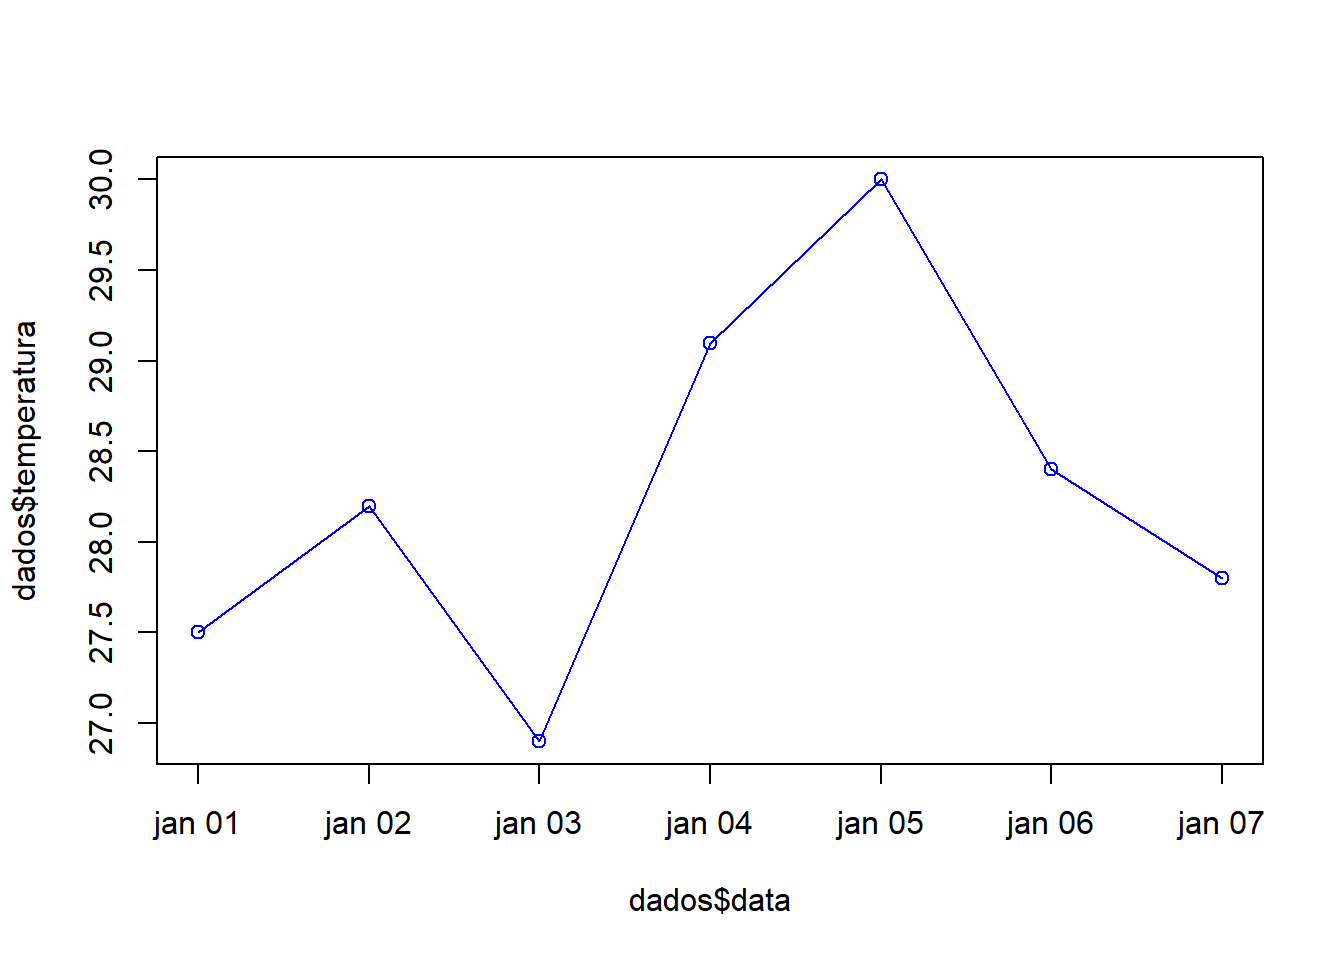
\includegraphics[keepaspectratio]{capitulos/01-introducao_files/figure-pdf/unnamed-chunk-1-1.pdf}}

\bookmarksetup{startatroot}

\chapter{Capítulo 2 -- Fundamentos de
Programação}\label{capuxedtulo-2-fundamentos-de-programauxe7uxe3o}

\section{Variáveis e Tipos de
Dados}\label{variuxe1veis-e-tipos-de-dados}

\subsection{Em R:}\label{em-r}

\begin{Shaded}
\begin{Highlighting}[]
\NormalTok{nome }\OtherTok{\textless{}{-}} \StringTok{"Maria"}
\NormalTok{idade }\OtherTok{\textless{}{-}} \DecValTok{21}
\NormalTok{temperatura }\OtherTok{\textless{}{-}} \FloatTok{27.5}
\NormalTok{chuva }\OtherTok{\textless{}{-}} \ConstantTok{TRUE}
\end{Highlighting}
\end{Shaded}

\section{Estruturas Condicionais}\label{estruturas-condicionais}

\begin{Shaded}
\begin{Highlighting}[]
\NormalTok{x }\OtherTok{\textless{}{-}} \DecValTok{25}
\ControlFlowTok{if}\NormalTok{ (x }\SpecialCharTok{\textgreater{}} \DecValTok{20}\NormalTok{) \{}
  \FunctionTok{print}\NormalTok{(}\StringTok{"Está quente"}\NormalTok{)}
\NormalTok{\}}
\end{Highlighting}
\end{Shaded}

\begin{verbatim}
[1] "Está quente"
\end{verbatim}

\bookmarksetup{startatroot}

\chapter{Capítulo 3 -- Estruturas de
Dados}\label{capuxedtulo-3-estruturas-de-dados}

\section{Vetores / Listas}\label{vetores-listas}

\begin{Shaded}
\begin{Highlighting}[]
\NormalTok{temperaturas }\OtherTok{\textless{}{-}} \FunctionTok{c}\NormalTok{(}\FloatTok{25.2}\NormalTok{, }\FloatTok{26.1}\NormalTok{, }\FloatTok{27.0}\NormalTok{, }\FloatTok{26.8}\NormalTok{)}
\NormalTok{temperaturas[}\DecValTok{2}\NormalTok{]}
\end{Highlighting}
\end{Shaded}

\begin{verbatim}
[1] 26.1
\end{verbatim}

\section{Data Frames}\label{data-frames}

\begin{Shaded}
\begin{Highlighting}[]
\NormalTok{dados }\OtherTok{\textless{}{-}} \FunctionTok{data.frame}\NormalTok{(}
  \AttributeTok{dia =} \DecValTok{1}\SpecialCharTok{:}\DecValTok{4}\NormalTok{,}
  \AttributeTok{temperatura =} \FunctionTok{c}\NormalTok{(}\FloatTok{25.2}\NormalTok{, }\FloatTok{26.1}\NormalTok{, }\FloatTok{27.0}\NormalTok{, }\FloatTok{26.8}\NormalTok{)}
\NormalTok{)}
\end{Highlighting}
\end{Shaded}





\end{document}
